%% vvase manual.tex

\documentclass[oneside]{memoir}
\usepackage{graphicx}
\usepackage[hidelinks]{hyperref}
%\usepackage{framed}
\usepackage{xcolor}
\usepackage{manual}
\usepackage[super]{nth}

%\usepackage{amsmath}
%\usepackage{amsfonts}
%\usepackage{amssymb}
%\usepackage{mathtools}

\begin{document}

\frontmatter
\chapterstyle{chappell}% This one is OK, but if we wrote our own we could probably do better
\pagestyle{empty}

% Title page
\vspace*{\fill}
\begin{center}
\HUGE\textsf{\VVASE{}}\par
\end{center}

\begin{center}
\Huge\textsf{User's Guide}\par
\end{center}

\begin{center}
\LARGE\textsf{Kerry Loux}\par
\medskip
\normalsize\textsf{version \version}\par
\end{center}
\vspace*{\fill}

\clearpage

% Copyright/license page

% TODO:  Put license info here

\begingroup
\footnotesize
\setlength{\parindent}{0pt}
\setlength{\parskip}{\baselineskip}
\textcopyright{} 2007-2015 Kerry R. Loux \\
All rights reserved

\begin{center}
\begin{tabular}{ll}
v0.8b:   & 29 July 2009 \\
v0.12a:  & 30 July 2015 \\
\end{tabular}
\end{center}
\endgroup

\clearpage

\pagestyle{headings}

\tableofcontents
\setlength{\unitlength}{1pt}
\clearpage
%\listoffigures
%\clearpage
%\listoftables
%\clearpage

\pagestyle{ruled}

\chapter{Preface}

I first became interested in vehicle dynamics through involvement with my college Formula SAE team.  I was on summer break after finishing my freshman year, and somehow I stumbled upon the team's website.  Racecars!  Cool!  So the next weekend, after some e-mails back and forth, I set out to a local autocross where the team was cooking burgers and hot dogs as a fundraiser.  Cars of all kinds racing through a sea of orange cones.  Having never been to an autocross before, I was curious.  ``Why is it that some cars lift the front wheel in the corners, and others lift the rear wheels?''  ``How come the real racecars don't screech tires like the street cars do?''

It didn't take long before it was clear that I had caught the racecar bug.  I was particularly drawn to suspensions.  I'm not entirely sure why that was, maybe because you could see all of the moving parts, or maybe because there was an experienced alumni who spent a lot of time in the shop who was also interested in suspension design.  Anyway, we spent many hours discussing vehicle dynamics and suspension design, pouring through the team's library of reference material and studying suspension kinematics with the help of purpose-built commercially available software.

The software we were using had terrible graphics and was somewhat tedious to use, but it provided accurate results and was simple enough to be confident that we provided the correct input.  It only permitted kinematic analysis of the suspension, and only one end of the car at a time, but it seemed well suited to our needs.  As I gained more experience and started to search for justification of more design decisions, it became clear that this software had some shortcomings.  At the time, it was our only option and many of the other engineering packages we used also had shortcomings.  Most of the time, it was easy to accept the issues and work around them.

In the summer of 2005, immediately following the conclusion of the 2005 FSAE season, a good friend of mine, Matt Jarvis, began work on redesigning the frame to be stiffer and lighter.  Matt was (and still is) a brilliant engineer.  Among his interests were programming, finite element analysis and composites.  He had taken the lead on the bodywork the previous year and wanted to consider adding composite panels to the frame design.  We had previously used aluminum panels for this purpose, bonding and riveting them to the frame.  Matt knew that a composite solution could improve the design, but it introduced several variables that we hadn't had to consider before.

Traditionally, someone would create a finite element model of the frame and apply a virtual torsional load.  The displacement was calculated by the finite element software from which a stiffness could be calculated.  The stiffness was compared to the weight to determine the overall quality of the design.  Then the designer would look at the stresses in the frame members and adjust the geometry and/or the cross section of certain members, with the goal of improving stiffness and reducing weight.  This process would continue until the designer stopped making progress or ran out of time.  Then they'd just pick the frame that had the best stiffness to weight ratio, and start fabrication.

Matt looked at this problem and saw all of the available permutations.  Even if you assumed the geometry was fixed, the number of frame members multiplied with the number of available cross sections (round, square, rectangular, dimensions, wall thickness) meant there was an incredible number of possible combinations.  He wrote VBA macros into excel spreadsheets that implemented a genetic search algorithm to intelligently evaluate a huge number of these permutations and hopefully converge on a solution.  After commandeering the computer lab overnight to run the optimization in parallel on some 20 machines, nearly 100,000 frame designs had been simulated.  The best design was both stiffer and lighter than the best human-designed frame from the previous year.  I was incredibly impressed by his success.

Also for the 2005-06 FSAE season, we decided to set the springs and dampers side-by-side instead of using coil-overs in an attempt to reduce the bending load on the damper shafts.  In theory, this would reduce friction in the damper and give us more control over the damping characteristics of the suspension.  This meant spending twice as much effort at each end to ensure the bellcrank geometry gave us the desired installation ratios across the entire range of motion.  Unfortunately, this was also one of the more tedious jobs to tackle with our suspension kinematics software.  Ideally, the designer would be able to look at the bellcrank along it's pivot axis, giving a clear view of the angles between the pushrod, bellcrank and spring or damper, and how they change through the range of motion.  Or better yet - show a plot of the installation ratio across the desired range of motion, updated dynamically as the bellcrank design was adjusted.  Also, it is important that all of these points lie on a common plane.  Our suspension package did not permit either of the above.  Our work-around was to bounce back-and-forth between our CAD software and the suspension design software.  This was not going to be a fun task.

After spending several hours trying to work out the bellcrank geometry, I thought I would try to solve the kinematics problem myself, creating a tool that was designed exactly for the problem at hand.  A few hours later, I had written some VBA code in an Excel spreadsheet that elegantly solved the problem of designing bellcrank geometry.  Even with the time invested in the creation of the tool, the total time to design new bellcranks had been reduced and the results were probably better than what would have been achieved with our prior workflow.  I experienced a great feeling of satisfaction, attached more to the creation of a useful tool than completing the design of the bellcranks.

Following my success with my bellcrank spreadsheet, I became interested in attempting to simulate the dynamics of the entire racecar.  With good tire data and mass properties data, we could simulate the car performing maneuvers and quantify how changes in \emph{anything} would affect lap times.  In December 2005 I took a stab at writing software that would model a full vehicle - tires, suspension, engine, brakes, etc.  I was extremely naive and this effort stopped only weeks after it started.  It would have been a much better use of my time to focus on the manufacturing of our racecar (apologies to my 2005-06 team members!).

\begin{figure}
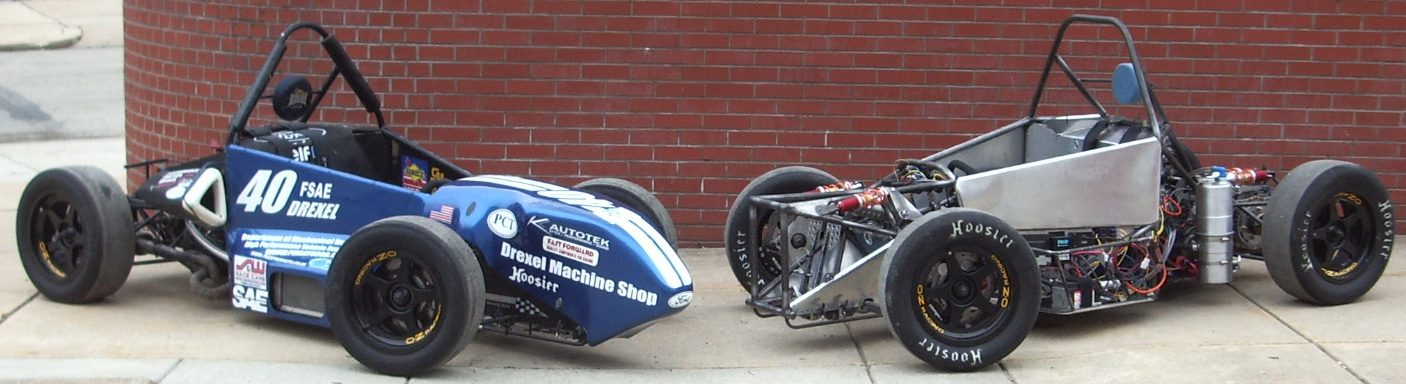
\includegraphics[width=\textwidth]{images/04-05cars}
\caption{The 2004 and (incomplete) 2005 Drexel University entries into the Formula SAE competitions}
\centering
\end{figure}

After graduating in 2007, I began work on what became the first incarnation of \vvase{}.  It was a simple application that could solve the vehicle kinematics problem for double A-arm suspensions.  I had made some improvements over the bellcrank spreadsheet I created a couple years earlier - it was faster, more accurate and more robust.  But it didn't do anything more than what other commercially available suspension kinematics software could do - in fact, in most ways it did less.  It was a learning exercise for me, but it wasn't very valuable as a tool.

At some point, I thought back to the genetic search algorithm that Matt had used to optimize the frame design.  Could something similar be applied to suspension kinematics?  After some careful thought and many hours of programming, I finally had something that was unique.  As far as I knew, there was no commercially available suspension kinematics package that could do an optimization like \vvase{}.

Although I never pursued a job in the auto industry, my FSAE experience became a significant influence on my career.  In addition to my engineering tasks associated with delivering our products, I develop special-purpose software tools for solving problems unique to our products and workflows.  I still have an interest in vehicle dynamics and racing, but I was surprised to find that I have a passion for creating tools.  This passion is what has driven me to continue work on \vvase{}, years after it began as an exercise and an experiment.  I hope that it satisfies other's needs to analyze suspension kinematics in the same manner it has satisfied my desire to create a tool.

% Influence of this experience on work (CAD tools, simulation, etc.)
% Influence of work experience back on this

%engineering problems are broad
%software is powerful and flexible, but requires expertise in both field and s/w usage.  confidence in inputs, confidence in output interpretation

%better decisions faster

\needspace{4\baselineskip}
\begin{flushright}
Kerry R. Loux \\
Langhorne, PA \\
July 2015
\end{flushright}

\chapter{Introduction} \label{ch:introduction}

%\vvase{} was designed as a tool that could be useful throughout the process of designing and testing a vehicle.  The vision was a single product that could perform kinematic analysis, dynamic simulation, process tire data and replay recorded data.

\vvase{} is a tool for analyzing suspension kinematics.  Given the locations of the suspension linkages and the kinematic state of the vehicle (pitch, roll, heave and steer), many output values are computed.  These outputs are key indicators of suspension performance and vehicle handling qualities.

There are other tools available that peform similar functions, but \vvase{} was designed with two unique features that make it stand out.

First, \vvase{} was designed to ease the process of evaluating differences between design options.  Always visible is a panel that displays the differences between all open car files for the specified kinematic state.  Additionally, iteration files can be used to compare kinematic outputs across a range of kinematic states - simultanously for as many car files as desired.  The iterations and panel displaying the kinematic outputs update continuously as suspension hardpoints are varied.

Second, \vvase{} provides a unique facility for performing complex optimizations.  These optimizations are based on a genetic search algorithm that allows the user complete control over the optimization process.  Genetic search algorithms allow broad coverage of highly non-linear solution spaces and can help avoid getting trapped at local minima.  In suspension design, moving a single hardpoint can affect many output paramters.  An optimization tool that balances multiple constraints is invaluable.

Currently, \vvase{} is limited to cars employing a double A-arm suspension at both ends.  It supports several spring/damper attachment methods, U-bar and T-bar anti-roll bars, asymmetric suspensions and several other configuration options that allow virtually any double A-arm suspension to be modeled.


\mainmatter

\chapter{Getting Started} \label{ch:gettingStarted}

\section{Installation} \label{sec:installation}

\vvase{} does not include any installation process or changes to the machine registry.  Simply place the executable and the pdf manual into the same directory.  After running the first time, any changes to the default settings are saved to a configuration file which will appear in the directory from which the application is run.

\section{Overview} \label{sec:overview}

Upon starting \vvase{} for the first time, the screen will look like Fig.~\ref{fig:defaultStartup}.  

\begin{figure}
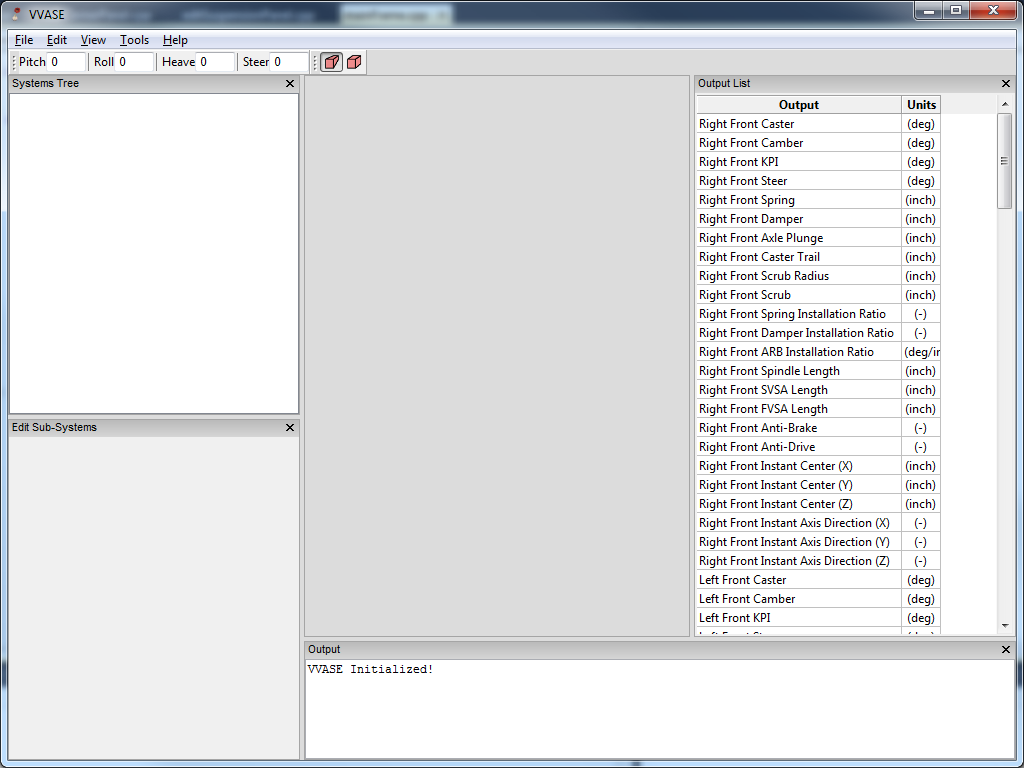
\includegraphics[width=\textwidth]{images/defaultStartup} \label{fig:defaultStartup}
\caption{Default screen configuration}
\centering
\end{figure}

\subsection{Systems Tree} \label{ssec:systemsTree}
\subsection{Edit Panel} \label{ssec:editPanel}
\subsection{Output List} \label{ssec:outputList}
\subsection{Output Pane} \label{ssec:outputPane}
\subsection{Main Display Area} \label{ssec:mainDisplayArea}
\subsection{Kinematics Toolbar} \label{ssec:kinematicsToolbar}
\subsection{3D Toolbar} \label{ssec:3DToolbar}

\section{Options} \label{sec:options}

\begin{figure}
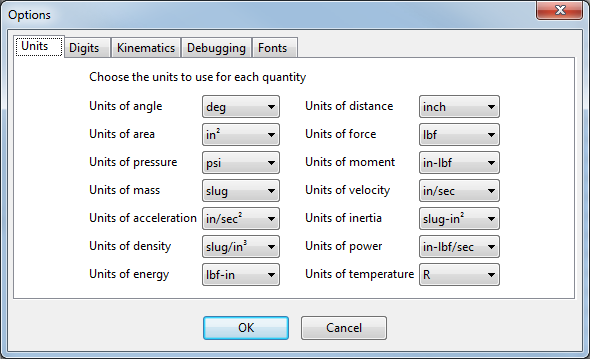
\includegraphics[width=\textwidth]{images/optionsUnits} \label{fig:optionsUnits}
\caption{Units options}
\centering
\end{figure}

\begin{figure}
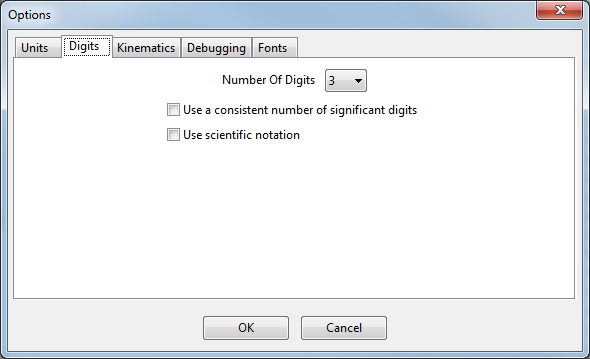
\includegraphics[width=\textwidth]{images/optionsDigits} \label{fig:optionsDigits}
\caption{Digits options}
\centering
\end{figure}

\begin{figure}
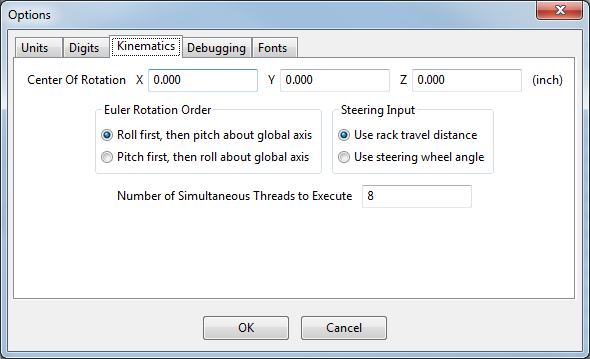
\includegraphics[width=\textwidth]{images/optionsKinematics} \label{fig:optionsKinematics}
\caption{Kinematics options}
\centering
\end{figure}

\begin{figure}
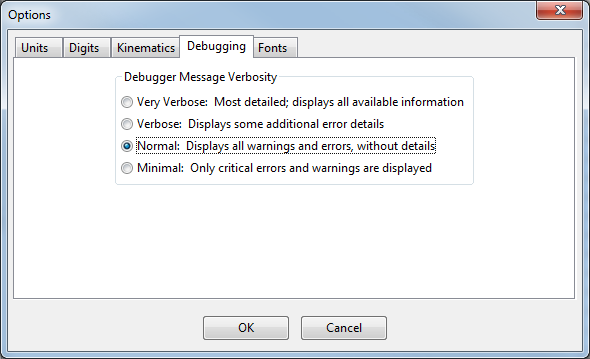
\includegraphics[width=\textwidth]{images/optionsDebugging} \label{fig:optionsDebugging}
\caption{Debugging options}
\centering
\end{figure}

\begin{figure}
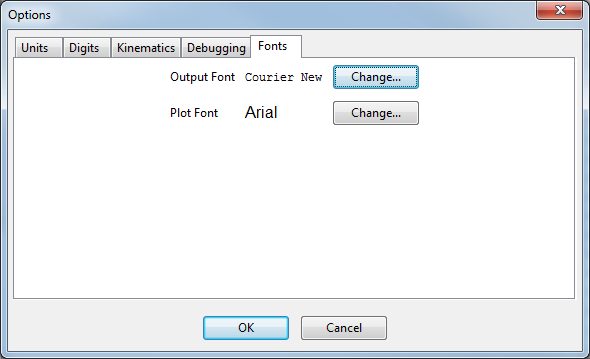
\includegraphics[width=\textwidth]{images/optionsFonts} \label{fig:optionsFonts}
\caption{Fonts options}
\centering
\end{figure}
\chapter{Cars} \label{ch:cars}

Vehicles in \vvase{} are represented by .car files.  These files store all information that describes the vehicle itself, including suspension hardpoints, mass properties, etc.

When a new vehicle is created, defaults values for all properties are created such that the suspension takes a reasonable form.  This makes it easier to associate hardpoint names with the points shown on-screen.

When a car file is active, the \element{Main Display Area} contains a 3D rendering of the tires and suspension elements.  This rendering is described in \sref{sec:3dCarDisplay}.

Car files create several subsystems in the \element{Systems Tree}, with each subsystem having unique \element{Edit Panel} content.  These subsystems are described in \sref{sec:subsystems}.

\section{3D Car Display} \label{sec:3dCarDisplay}

The 3D vehicle rendering shows the locations of all of the suspension elements and tires in the specified kinematic state.  An example of the 3D rendering of a car is shown in \figref{fig:car}.  In the rendering, the green vectors represent roll centers and roll axes, and yellow vectors represent instant centers and instant axes.

\begin{figure}
  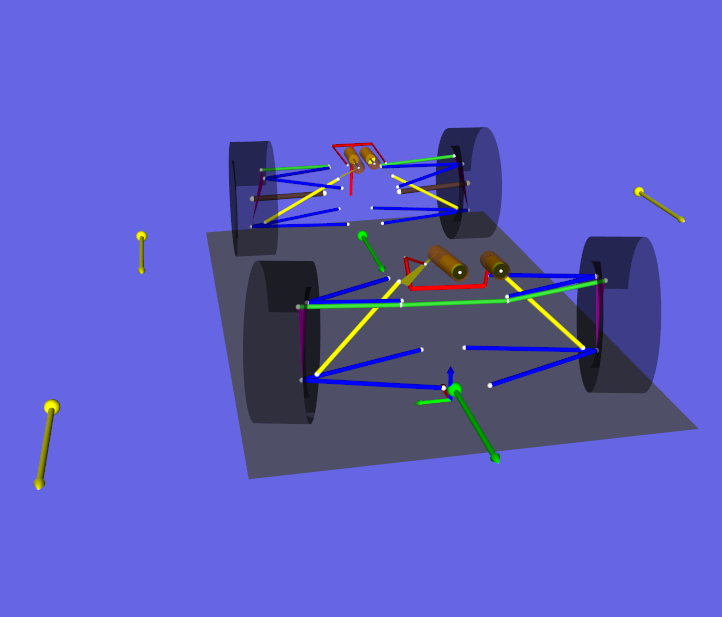
\includegraphics[width=\textwidth]{images/car}
  \caption{Example 3D car rendering for a kinematic state including roll and steer inputs} \label{fig:car}
  \centering
\end{figure}

It is possible to interact with the 3D display by clicking and dragging with the mouse to rotate, or using the mouse wheel to zoom.

By default, cars are rendered in perspective mode, but the \element{3D Toolbar} can be used to toggle between perspective and orthographic modes.  See \sref{ssec:3DToolbar} for more information.

The appearance of all of the suspension elements can be adjusted by clicking on the \element{Car} menu, and then selecting \button{Appearance Options}.  The color and size can be adjusted and the visibility of any object can be toggled on or off.  Resolution, which can also be adjusted, corresponds to the number of triangles used to approximate round objects during the rendering process.

When a hardpoint is selected in the \element{Edit Panel}, a ``helper orb'' is drawn, which highlights the selected point in the 3D display.  This can be helpful in understanding the naming of each hardpoint.

\section{Subsystems} \label{sec:subsystems}

Each car file includes several subsystems.  These subsystems can be accessed by expanding the active car in the Systems Tree.  The subsystems are described below.

\subsection{Aerodynamics} \label{ssec:aerodynamics}

This subsystem is currently unused.

\subsection{Brakes} \label{ssec:brakes}

The brakes subsystem includes three parameters that affect the calculated kinematic outputs.  These parameters are toggled to indicate whether or not the front and rear brakes are inboard or outboard, and the portion of the braking effort that can be expected to come from the front tires.  These parameters affect the calculation of the front anti-dive and rear anti-lift.

\subsection{Drivetrain} \label{ssec:drivetrain}

This subsystem is currently unused.

\subsection{Engine} \label{ssec:engine}

This subsystem is currently unused.

\subsection{Mass Properties} \label{ssec:massProperties}

There are several mass properties parameters associated with each car file.  For kinematics analysis, only the z-component of the center of gravity is currently used.  It affects only the calculation of the anti-dive and anti-lift values.

%For quasi-static analysis, all parameters except for the inertia tensor are used.

\subsection{Suspension} \label{ssec:suspension}

The suspension is the heart of the kinematics analysis.  This is where all of the suspension hardpoints are defined, as well as a number of other suspension geometry settings.  By default, the suspensions are assumed to be symmetric, but unchecking the corresponding option on the \element{Suspension} tab creates a separate additional tab for each corner instead of the \element{Front} and \element{Rear} tabs that exist by default.  Also on the \element{Suspension} tab are options for the type of anti-roll bar present at each end (if any) and whether or not \nth{3} springs are present at each end.  Depending on the selected anti-roll bar and \nth{3} spring options, a list of hardpoints may be displayed in the grid at the top of the panel.  These hardpoints can be edited by typing in new values in this grid.  Clicking on the hardpoint will highlight the corresponding point in the 3D display.

The additional tabs, whether there are two or four, are identical.  Each tab corresponds to a corner or a pair of corners at one end of the car and includes a list of hardpoints, spring/damper options and static toe and camber settings.  Just as with the \element{Suspension} tab, selecting a hardpoint in the list will highlight the corresponding hardpoint(s) in the 3D display.

By default, both ends of the car have pushrod suspensions.  By changing the \element{Attachment} to the \selection{Upper A-Arm} or a high location on the \selection{Upright} and modifying the bellcrank hardpoints, pullrods can also be modeled.  Outboard spring/damper units and rocker arms can be modeled by selecting the \selection{Outboard/Rocker} \element{Actuation Type}.

Static toe and camber settings affect only the calculated steer and camber values.

\subsection{Tires} \label{ssec:tires}

The diameter, width and stiffness of all four tires may be specified individually.  The width is for display purposes only.  The diameter affects the tire rendering as well as the kinematic calculations.  For the purposes of the kinematics analysis, the tires are assumed to be thin, rigid disks.  For all kinematic states the tires are assumed to rest on the ground.

For quasi-static analysis, the the tire stiffness parameters are used to compute tire deflections.  The rendering will still draw perfectly round tires, which will result in the tire being drawn slightly below the ground plane.

\chapter{Iterations} \label{ch:iterations}

Iteration objects provide a means of plotting kinematic outputs across a range of kinematic states.  The settings for these plots are stored in .iteration files.

When a new iteration is created, default settings for the iteration are loaded from the configuration file.  These defaults can be configured by the user (see \sref{sec:optionsTab}).

When an iteration file is active, the \element{Main Display Area} contains a rendering of the plot, as configured by the user.  The user can interact with the plot and perform mathematical operations on plotted data.  More information is in \sref{sec:plotDisplay} below.

Also when selected, the Edit Panel will contain three tabs.  These tabs are described in \sref{sec:rangeTab}-\ref{sec:optionsTab} below.

Behavior of the iteration can be further customized by using the options provided in the \element{Iteration} menu, which is described in \sref{sec:iterationMenu}.

\section{Plot Display} \label{sec:plotDisplay}

The plot is displayed in the \element{Main Display Area}.  Below the plot is a list of all of the active plots.  Here, curves can be toggled on/off or optionally plotted against the right y-axis instead of the left.  The color, size and marker size for each curve can be independently adjusted.  Right-clicking on the plot are or the plot list will generate a context-sensitive pop-up menu.  These pop-up menus provide a means of performing mathematical operations on plotted data, fitting curves to plotted data, changing plot background colors, toggling the legend on or off and more.  The legend can be dragged and dropped to place it in the plot area as desired.  Double-clicking in the plot area introduces a cursor, which can be dragged across the extents of the plot area.  The values corresponding to places where the cursor crosses the plot curves are displayed in the grid below the plot area.

An example of an iteration plot is shown in \figref{fig:iteration}.

\begin{figure}
  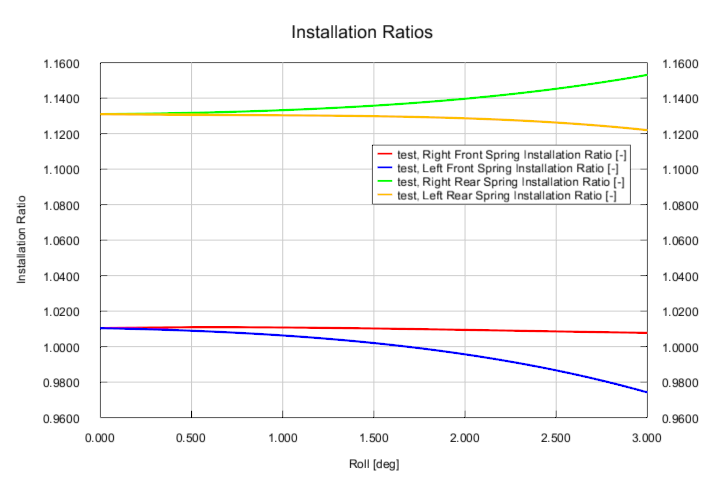
\includegraphics[width=\textwidth]{images/iteration}
  \caption{Example iteration Plot Display showing the installation ratios at all four corners of a vehicle while experiencing roll} \label{fig:iteration}
  \centering
\end{figure}

\section{Range Tab} \label{sec:rangeTab}

The \element{Range} tab describes the range of kinematic states which are to be represented on the plot.  Any combination of pitch, roll, heave and steer can be used as start and end conditions.  The number of points used on the plot can also be adjusted.  Generally, kinematic outputs change slowly and smoothly with respect to the kinematic states.  For these cases, smooth curves can be produced with a relatively few number of points.  Occasionally, however, an output will appear to change rapidly and more points are required to produce a smooth curve.  It is advisable to use as few points as possible, especially if the iteration is to be associated with several open car files, as each additional point requires another sequence of calculations for each associated car.

\section{Active Plots Tab} \label{sec:activePlotsTab}

The \element{Active Plots} tab allows the user to specify which outputs should be plotted in the active iteration file.  It is possible to select as many outputs for plotting as desired.

\section{Options Tab} \label{sec:optionsTab}

The \element{Options} tab allows the user to manually specify the plot title and axis labels.  There is also an option that permits toggling the grid lines on and off.

At the bottom of the panel is a button labeled \button{Set As Default Properties}.  Clicking this button will save all of the current plot configuration options to the configuration file.  Each time a new iteration file is created, this configuration will be applied.

\section{Iteration Menu} \label{sec:iterationMenu}

All iteration data is exportable into a .csv format which can be opened with Microsoft Excel or other tools.  This can be done by selecting the \button{Export Data} entry in the \element{Iteration} Menu.

By default, iterations auto-associate with all open car files.  This means that the desired kinematic outputs are plotted for every open car.  This makes side-by-side comparisons of different geometries easy.  If this is not desired, the \button{Associated Cars} entry in the \element{Iteration} menu can be used to specify which cars should be analyzed by the iteration file.

\vvase{} will automatically select the correct independent variable for the plot when only a single kinematic input is varied.  For cases when multiple kinematic inputs are varied, the user can select the independent variable by selecting the \element{Set X-Axis} entry in the \element{Iteration} menu.

\chapter{Optimizations} \label{ch:optimizations}


% Other chapter styles, possible for future use
%\appendix
%\backmatter

\end{document}